\section{Dataset Creation}
As already mentioned, the Dataset has been created with Matlab And FEMM. It was possible to create a script that simulates in \gls{fem} a randomly generated electric motor, and measure the magnetic field inside the magnets to check for demagnetization.

Thanks to Giacomo Sala, professor of Electric Motor Design at MUNER\cite{MUNER}, that provided to the students the code to easily simulate an electric motor using FEMM and Matlab.
\begin{figure}[H]
    \centering
    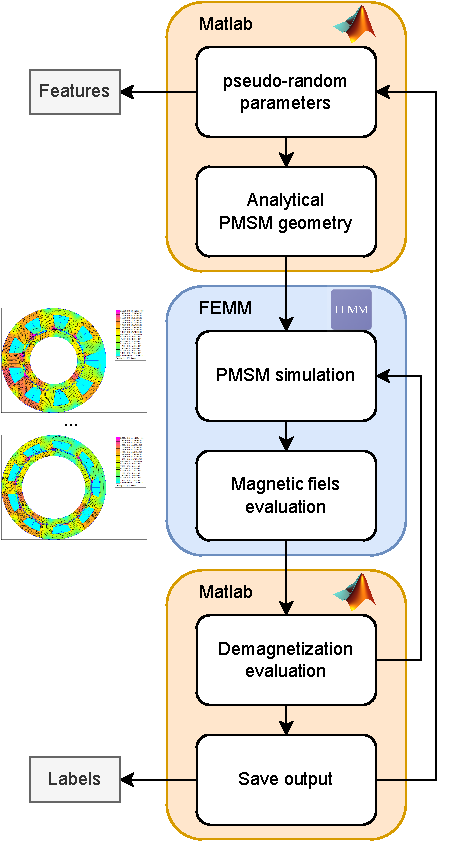
\includegraphics[width=0.54\textwidth]{sections/images/section2/dataset_creation.pdf}
    \caption{Dataset creation workflow}
    \label{fig:dataset_creation}
\end{figure}
The main steps of the dataset generation process are summarized in \cref{fig:dataset_creation}. In greater details the steps are:
\begin{enumerate}\label{tab:dataset_creation}
    \item Pseudo randomly generate the motor parameters and values, to be used as \emph{features}.
    \item Generate the motor geometry analytically.
    \item Run \gls{fem} simulation of the motor.
    \item Measure the magnetic field inside the magnets, and extrapolate the point where field is maximum.
    \item Compare the measured field to its maximum possible value $H_{CI}$.
    \item Repeat measurements until demagnetization happens.
    \item Save the last "safe" current overload value that will not create overload as a \emph{label}.
\end{enumerate}
\subsection{Features}
Features have been pseudo randomly generated: a known working motor configuration has been chosen, where some parameters (the features) have been changed randomly in a specific range.

It was not possible to chose the features completely randomly, or some motor configuration could have been physically impractical.

The features, and their range, are:
\begin{center}
    \begin{table}[H]
       \renewcommand{\arraystretch}{1.2}
        \centerline{
        \centering
        \begin{tabular}{|r|c|c|c|}
        \hline
        &Feature & Mean value & Range \\
        \hline
        $T_{spec}$&Nominal Torque&\SI{150}{\newton\metre}&$\pm$ \SI{75}{\newton\metre}\\
        \hline
        $W_{spec}$&Rated Speed&\SI{3.5}{\kilo\rpm}&$\pm$ \SI{1.75}{\kilo rpm}\\
        \hline
        $B{mr}$&Magnetic Loading&\SI{0.75}{\tesla}&$\pm$ \SI{0.375}{\tesla}\\
        \hline
        $\delta$&Electric Loading&\SI{4}{\kilo\ampere/\metre}&$\pm$ \SI{2}{\kilo\ampere/\metre}\\
        \hline
        $m$&Aspect Ratio&\SI{1.5}{}&$\pm$ \SI{0.75}{}\\
        \hline
        $S_o$&Slot Opening&\SI{5}{\milli\metre}&$\pm$ \SI{1.75}{\milli\metre}\\
        \hline
        $d_0$&Airgap Thikness&\SI{1.2}{\milli\metre}&$\pm$ \SI{0.42}{\milli\metre}\\
        \hline
        $l_{magn}$&Magnet height&$l_{magn0}$ from calculation&$l_{magn0}*1.5\pm l_{magn0}*0.1$\\
        \hline
        $h_4$&Slot Opening height&\SI{2}{\milli\metre}&$\pm$ \SI{0.7}{\milli\metre}\\
        \hline
        $h_3$&Wedge Height&\SI{5}{\milli\metre}&$\pm$ \SI{1.75}{\milli\metre}\\
        \hline
        \end{tabular}}
        \caption{Features summary}
    \end{table}
\end{center}
\subsubsection{Note on \texorpdfstring{$l_{magn}$}{Lmagn} }
The only feature that has not chosen like the others is the magnet height $l_{magn}$. This because $l_{magn}$ needs to be greater than a certain quantity (dependent on other chosen features), so it was not possible to randomize it from a given value. To make the output result of the simulations more interesting, it has been decided to increase the calculated value $l_{magn0}$ by $1.5$, and to randomize this last value: doing so, it was possible to see more variegate values of maximum overload in output.

If $l_{magn}$ was chosen only considering the initial calculation, we would have seen a lot of low overload value, and the labels would have been much less interesting.
\subsection{Labels}
Each simulation outputs a single label $OL_{max}$: a number which represents the maximum overload that the motor is capable before demagnetizing.
\subsubsection{Magnetic field \texorpdfstring{$H_{magn}$}{Hmagn} measurement}
The magnetic field is measured in \gls{fem} simulation along the perimeter of a circumference that touches the mean height of the magnet: an example can be seen as the red line in \cref{fig:measurment_line}
\begin{figure}[H]
    \centering
    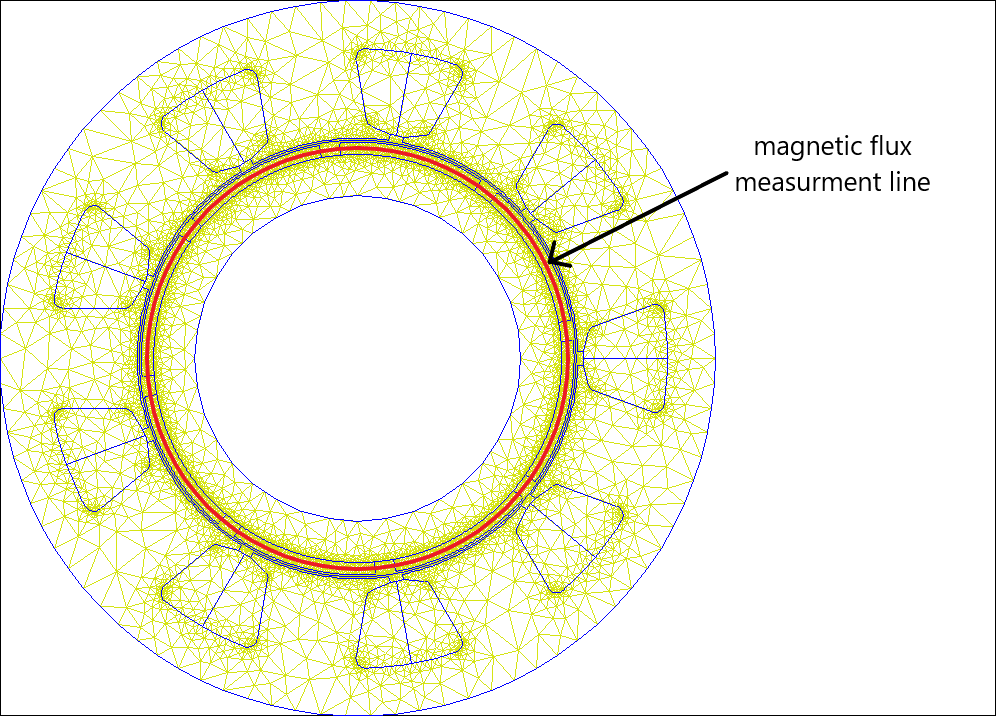
\includegraphics[width=0.6\textwidth]{sections/images/section2/measurment_line.png}
    \caption{Magnetic field measurement line example}
    \label{fig:measurment_line}
\end{figure}
\subsubsection{Maximum overload detection}
The overload detection and the labels output follows the following scheme:
\begin{enumerate}
    \item Matlab script starts by simulating the motor at nominal current.
    \item The maximum value of magnetic field along that line is find.
    \item Check if $|H_{magn}|<|H_{CI}|$.
    \item If the check is \textbf{true}: no demagnetization is happening, reiterate the simulation with increased current.
    \item If the check is \textbf{false}: demagnetization is happening, stop the simulation, save the last overload value as the label (that \gls{ol} will be the last one before demagnetization).
\end{enumerate}
This cycle is repeated for all the simulated motors.
\subsubsection{Note on label value}
Labels value are in a range between $0$ and $11$, where $0$ means no overload, and $11$ represents an overload of $6.5$.

To get the overload value $OL$ from the output of the script, the following equation needs to be applied:
\begin{equation}
    OL = \frac{Label}{2}+1
\end{equation}